\documentclass[a4paper,english]{article}
\usepackage{graphicx}
\usepackage[T1]{fontenc}
\usepackage[utf8]{inputenc}
\usepackage{babel}
\usepackage{hyperref}
\usepackage{upgreek} %proper greek letters
\usepackage{fullpage}
\usepackage{lineno}
\usepackage{amsmath} % typesetting math
\usepackage{amssymb}
\usepackage{booktabs} % nice tables
\usepackage[round,sort&compress]{natbib}
\usepackage{pdfpages} %include external pdfs
\usepackage{enumitem} %for noitemsep in lists
\usepackage{csquotes} %for noitemsep in lists
\usepackage{subfig}
\renewcommand{\arraystretch}{1.2} % space in tables
\usepackage{authblk}
\usepackage[titletoc,title]{appendix} %for appendix titles
\usepackage[colorinlistoftodos,prependcaption,textsize=tiny]{todonotes} %todo note in margin

\begin{document}

\title{Comparison of Multi-Parallel Slit and Knife-Edge Slit Prompt Gamma Cameras in the context of hadrontherapy verification}

\author[1,2]{Brent F. B. Huisman}
\author[2]{É. Testa}
\author[1]{D. Sarrut}
\affil[1]{~CREATIS, Université de Lyon; CNRS UMR5220; INSERM U1206; INSA-Lyon; Université Lyon 1; Centre Léon Bérard, Lyon, France}
\affil[2]{~IPNL, Université de Lyon; CNRS/IN2P3 UMR5822; Université Lyon 1 Lyon, France}
\affil[ ]{~E-mail: brent.huisman@cern.ch}

\maketitle

\begin{abstract}

\emph{Purpose:} 

\emph{Materials and Methods:} 

\emph{Results:} 

\emph{Conclusion:} 

\end{abstract}


%%%%%%%%%%%%%%%%%%%%%%%%%%%%%%%%%%%%%%%%%%%%%%%%%%%%%%%%%%%%%%%%%%%%%%%%%%%%%%%%
\section{Introduction}

\paragraph{State of the art} At the moment, two papers have proposed a comparison of MPS-KES cameras:
\begin{itemize}
	\item Smeets 2016 Fontiers in Oncology: experimental comparison with a non-optimized MPS camera (CLaRyS designed with non-optimized geometrical parameters)
    \item Lin 2017 Radiation Physics and Chemistry : MC comparison with the MPS Korean design whose optimization procedure is actually questionable
\end{itemize}
In overall, the camera configurations present many parameters, namely geometrical parameters and event selections (especially energy deposition selection). Therefore, in principle, some theoretical expectations are required to set relevant parameters and to allow for a fair comparison of the two types of collimators. Although the aforementioned studies may give the impression to provide a fair comparison (use of the same absorbers, same beam-collimator and collimator-absorber distance in the case of Lin 2017), they do not provide a thorough justification of their sets of parameters. Surprisingly, some parameters are even not the same between the two camera types. While it can be understood in Smeets 2016 due to experimental constraints, it is more questionable Lin 2017 (different energy deposition selection).

\paragraph{Objectives}
The objectives of the present paper are the following:
\begin{itemize}
	\item Estimate the MPS and KES detection efficiencies and spatial resolution from geometrical considerations 
    \begin{itemize}
    	\item Draw some conclusions about the intrinsic features of MPS and KES collimators. 
        \item Estimate the MPS and KES performances in Smeets 2016 and Lin 2017: the KES/MPS detection efficiency ratio is 1.6 for Smeets 2016 and 5.3 for Lin 2017 (with the energy window)
        \item Definition of a set of parameters to allow for a fair MPS and KES comparison with MC simulations
    \end{itemize}
    \item Fair comparison of the types of collimators with MC simulations. 
    \begin{itemize}
    	\item same absorber (the LYSO absorber of the KES prototype that we can consider as the reference) with E> 1 MeV and without TOF
        \item geometry as close as possible to the prototypes: 
	\end{itemize}            
    \item Simulations of the two prototypes as they are published (results of the submitted paper with the \enquote{regular} cylindrical PMMA target of 15 cm diameter and 20 cm lenght). 
    \begin{itemize}
		\item the comparison of the two prototypes
		\item the identification of the impact of energy selection (>1 MeV vs 3-6 MeV selection for KES) and TOF (for MPS) although the latter has been already shown in Roellinghoff PMB 2014.
	\end{itemize}        
\end{itemize}



%%%%%%%%%%%%%%%%%%%%%%%%%%%%%%%%%%%%%%%%%%%%%%%%%%%%%%%%%%%%%%%%%%%%%%%%%%%%%%%%
\section{Materials and Methods}

%%%%%%%%%%%%%%%%%%%%%%%%%%%%%%%%%%%%%%%%%%%%%%%%%%%%%%%%%%%%%%%%%%%%%%%%%%%%%%%%
\subsection{Simulation}

Imaging paradigms such as PG detection are evaluated against experiments, and often also with Monte Carlo (MC) simulations~\citep{Moteabbed2011,Gueth2013,Robert2013,Golnik2014a,Janssen2014}. For rarely occurring processes such as PG simulation, convergence to the model of the truth to within acceptable statistical error can be slow. This paper presents an \emph{in silico} study of the feasibility of the clinical relevance of PG FOP estimation using collimated cameras, and uses the vpgTLE variance reduction method described in \cite{Huisman2016}. vpgTLE is a two stage process, where firstly a PG yield distribution image is estimated, which in the second stage is used as a PG source with which detectors can be investigated. Gate 7.2~\citep{Sarrut2014} with Geant 4.10.02 and the QGSP\_BIC\_HP\_EMY physics list, commonly used for PG studies, are used in this analysis. Thanks to vpgTLE, simulations for about $10^9$ protons (about $6\times10^8$ photons) took 1-2 hours on a single core of an Intel(R) Core(TM) i7-3740QM.

%%%%%%%%%%%%%%%%%%%%%%%%%%%%%%%%%%%%%%%%%%%%%%%%%%%%%%%%%%%%%%%%%%%%%%%%%%%%%%%%
\subsection{PG camera modeling}\label{sec:camera}

Two PG detectors tailored to FOP verification (illustrated in fig.~\ref{fig:detectors}) were chosen:
\begin{itemize}[noitemsep]
\item the CLaRyS multi-parallel-slit (MPS) camera, Case 1 \citep{Pinto2014a}
\item[] This camera intends to measure the whole PG profile to control ion-ranges in the patient with a field of view (FoV) of 300 mm. It makes use of ToF selection to reduce the neutron background. In the optimization carried out by \cite{Pinto2014a}, parameters such as collimator pitch, axis-to-collimator and axis-to-detector were varied, and their impacts evaluated in terms of fall-off retrieval precision (FRP) and spatial resolution (sharpness of the fall-off region). Here, configuration 1 (with relaxed constraints on spatial resolution) was chosen for its optimal FRP performance. As was done by \cite{Pinto2014a}, the camera lengths (collimator and scintillator volume) are chosen \emph{up to} 300 mm, such that the length is an integer multiple of the pitch size, with for the collimator a collimator-leaf-width extra, to ensure each pixel has a leaf on both sides. With the 8 mm pitch and 2.6 mm collimator-leafs, this results in a scintillator volume of length 296 mm and collimator length 298.6 mm.
\item the IBA knife-edge (KES) camera \citep{Perali2014,Sterpin2015}
\item[] The purpose of this camera consists of verifying the BP position with a FoV of 100 mm. \cite{Richter2016} provides the first clinically obtained results. At this time, no other camera has been subjected to clinical tests, which is why we consider this prototype a benchmark.
\end{itemize}

\begin{figure}[htp]
  \centering
  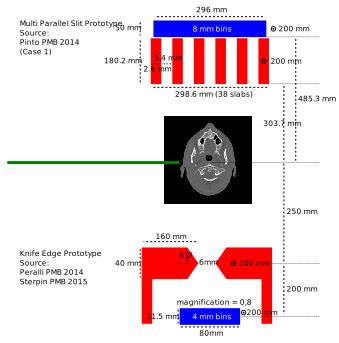
\includegraphics[width=0.9\linewidth]{detectors}
  \caption{Schematic presentation of the two PG cameras considered in this study. The green arrow represents the proton beam. In red the collimation elements and in blue detection elements. The dimensions were taken from \cite{Pinto2014a} and \cite{Perali2014,Sterpin2015}. Note that the two cameras have an identical detector height ($\odot$ symbol), the two cameras were positioned at an identical location above the head during all simulations, and that here they are not drawn to scale.}
  \label{fig:detectors}
\end{figure}

Regarding background ToF selection, for the IBA C230 accelerator with a period of 10 ns, \cite{Pinto2014a} chose a window of 4 ns around the PG maximum, based on experimental ToF spectra. This means that about 60\% of the noise could be removed. For the KES prototype ToF is not used, leading to a higher background, as is evident when one compares the backgrounds as published in the two publications. A second difference is the energy selection window. The IBA group employ a 3-6 MeV window, whereas the CLaRyS collaboration produced their optimization with a 1-8 MeV window. We will compare each camera with their published properties, that is to say: a 1-8 MeV window and ToF for MPS and a 3-6 MeV window without ToF for KES.

Both PG camera prototypes have different photodetectors and different detector electronics. In this study, these differences are not implemented. Instead, the method as described in \cite{Gueth2013} was used to obtain the interaction point of an impinging photon. If the integrated energy deposited in a crystal lies in the acceptable energy and ToF window, the event is recorded. The position of the event in the crystal is considered as the energy weighed barycenter of all interactions in the crystal, plus a random value taken from a 5mm FWHM Gaussian to simulate the electronics and the detector resolution.

%%%%%%%%%%%%%%%%%%%%%%%%%%%%%%%%%%%%%%%%%%%%%%%%%%%%%%%%%%%%%%%%%%%%%%%%%%%%%%%%
\subsection{Background estimation}

Background estimation in PG simulation is a difficult and largely unsolved issue \citep{Huisman2016,Sterpin2015,Pinto2014a,Perali2014}. Simulations would ideally include beam nozzle and whole room modeling, but these are habitually omitted. ToF selection techniques can improve the signal-to-noise ratio (SNR) \citep{Testa2008}, but then depend on the proper simulation of the beam accelerator time structure. As noted in \cite{Huisman2016}, no validation for background in PG simulations has been performed at this time. In this study, the stable time structure of current generation cyclotrons was assumed, in which the neutron background is largely constant. Estimates of background counts in the detector are taken from \cite{Pinto2014a,Perali2014}, which are both based on measured data:

\begin{itemize}[noitemsep]
\item MPS: \cite{Pinto2014a} fig.~9: $1 \cdot 10^{3} \pm 1 \cdot 10^{2}$ per $4\cdot10^9$ primary protons per 8 mm bin
\item[] Converted to per primary proton: $2.5 \cdot 10^{-7} \pm 0.25 \cdot 10^{-7}$
\item KES: \cite{Perali2014} fig.~11: $5 \cdot 10^{-7} \pm 0.5 \cdot 10^{-7}$ per primary proton per 4 mm bin
\end{itemize}

Per unit of bin length, the background yield of the MPS with ToF is therefore 4 times as low as the background seen with the KES.


%%%%%%%%%%%%%%%%%%%%%%%%%%%%%%%%%%%%%%%%%%%%%%%%%%%%%%%%%%%%%%%%%%%%%%%%%%%%%%%%
\subsection{Fall-off position estimation procedure}

From a clinical perspective, the range estimate could be more interesting than FOP, because it can distinguish simple offset errors from patient morphological change. While the MPS camera was conceived for whole range PG profile detection, the KES camera FoV was chosen for BP region PG detection only. To make the comparison fair, only the FOP could be considered. Multiple approaches to extracting a FOP from the line profile have been proposed \citep{Smeets2012,Gueth2013,Roellinghoff2014a,Janssen2014,Sterpin2015}. In preparatory work, a number of the proposed procedures were investigated. Significant sensitivity to free parameters on the final FOP estimates were seen. In summary, the FOP estimate depends greatly on the procedure, and often on having yields uncommon on the spot-level in clinical TPs, and also on an absence of unavoidable inhomogeneities.

Therefore the fitting method was not chosen as a topic for study in this paper. Instead, a simple method that works on most the data available to the authors was used: first a smoothed and interpolated spline function is fitted against the detected PG data points, after which a baseline and (distal) peak position are determined. The intersection of the spline with the half-height of the peak above the baseline is then taken as the FOP. A more detailed description of the procedure may be found in appendix~\ref{sec:fopproc}.

%%%%%%%%%%%%%%%%%%%%%%%%%%%%%%%%%%%%%%%%%%%%%%%%%%%%%%%%%%%%%%%%%%%%%%%%%%%%%%%%
\subsection{Spot grouping}

In particle therapy and particle therapy imaging literature often it is mentioned that a spread out Bragg Peak (SOBP) is achieved by giving the most distal iso-energy layer the highest weight and each successive iso-energy layer is of lower energy and of lower weight. This is correct when positions in the transverse plane (to the beam direction) are considered, for homogeneous phantoms, and when interpolation is not required. Interpolation happens when the energy levels of the beam delivery system do not correspond with the distal tumor contour \citep{0031-9155-57-21-N405}, in which case the dose contour is approximated by spreading the distal dose of the nearest two possible energies (see fig.~\ref{fig:planning}).

\begin{figure}[htp]
  \centering
  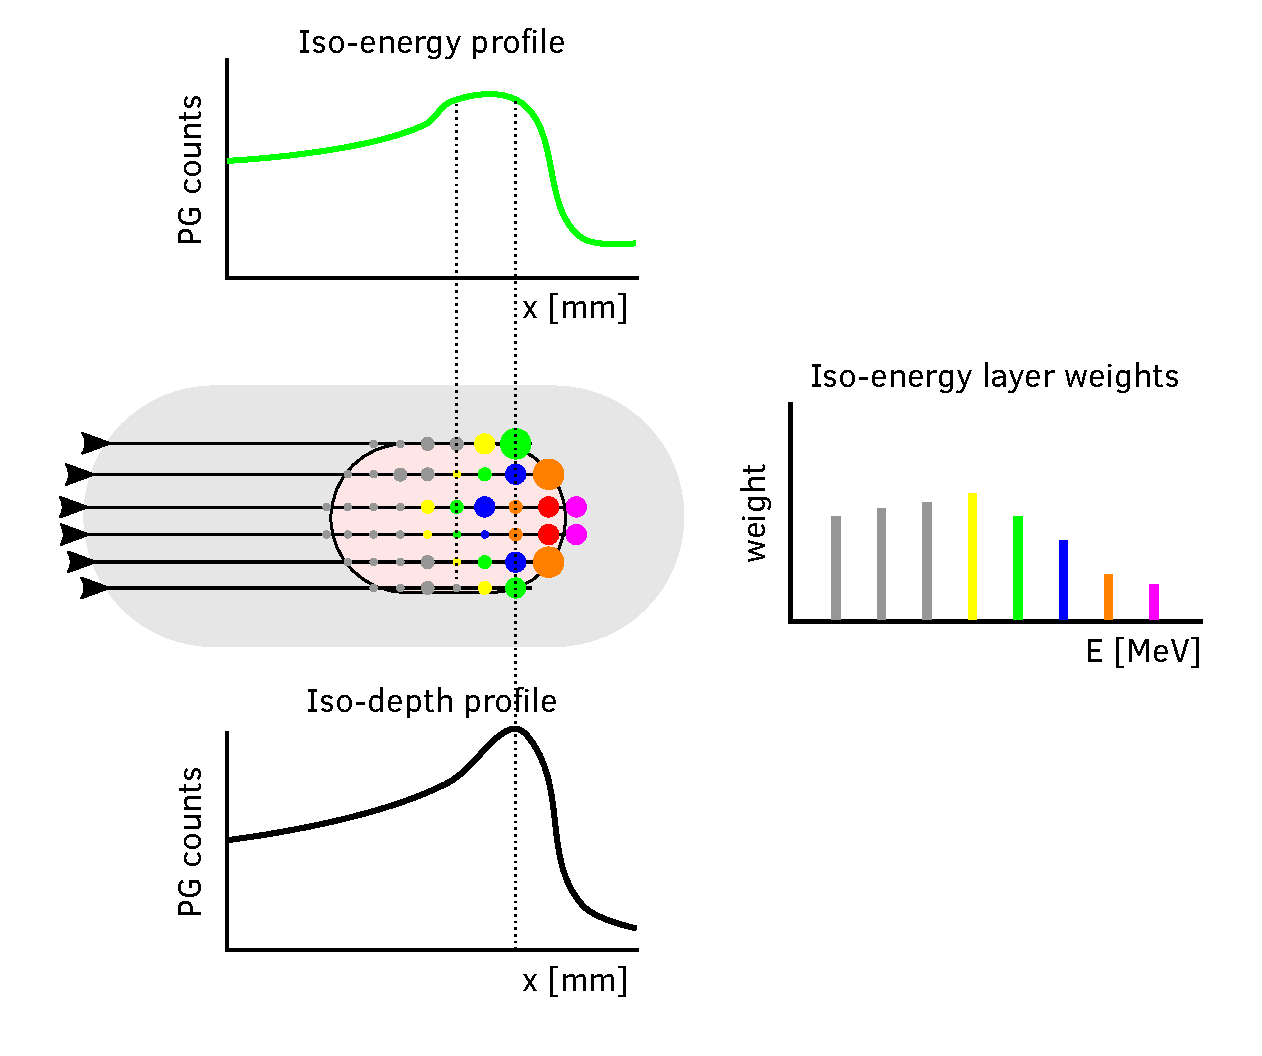
\includegraphics[width=0.6\linewidth]{planning}
  \caption{A schematic view of a patient (light gray), planned treatment volume (peach-pink), and a proton beam (black horizontal lines coming in from the left). Superimposed are various spots, where the size of the circles indicate spot weights. The spot colors indicate the iso-energy layer of which the spot is part. On the right, the weights (proton counts) per iso-energy layer are plotted, in similar fashion to fig.~\ref{fig:planmid}. On top, the PG profile is sketched for an iso-energy layer. On the bottom, the PG profile is sketched for iso-depth layer (spots of various color on the dotted line). In violet and red, the four dots on the distal end of the two most central beam lines, the effect of interpolation is illustrated: not always is every distal spot planned with a high weight.}
  \label{fig:planning}
\end{figure}

As established in section~\ref{sec:tpanalysis}, a difference was expected between the number of protons per spot as planned and sufficient for reconstruction. Depending on the beam line, the minimum unit of PG detection may be a spot (beam scanning) or an iso-energy layer (passive scattering). Since most new centers employ active beam scanning, new grouping methods are possible. Here a spot grouping method is proposed based on the notion of depth proximity. On the planning CT the 3D dose distribution is computed per spot, and then a dose FOP is determined with the same algorithm as for PG FOP. The FOPs for each spot are binned along the beam line, and these bins we call iso-depth layers. The assumption is that due to inhomogeneities, protons within an iso-energy layer may have very different FOPs in the patient. This iso-depth grouping method will be compared to grouping by iso-energy.


%%%%%%%%%%%%%%%%%%%%%%%%%%%%%%%%%%%%%%%%%%%%%%%%%%%%%%%%%%%%%%%%%%%%%%%%%%%%%%%%
\subsection{Figures of merit}\label{figmerit}

When evaluating a detector, principally the accuracy and precision are of interest: does the PG camera estimate the FOP correctly (accurate) and is the result reproducible (precise)? A more clinical point of view could be: does the detector correctly signal significant changes? A precise FOP estimate or FOP shift estimate is perhaps not required, but a correct indication of significant change \emph{is}.

Employing the batch method we realize between 20 and 50 simulations for each experiment, each resulting in a FOP estimate, giving us a mean $\upmu_\textrm{FOP}$ and a standard deviation $\upsigma_\textrm{FOP}$ for a certain experiment. Since we are studying the effect of replacing the CT with a RPCT to simulate patient change, we run each experiment with both CT and RPCT. Each FOP estimate of the N CT realizations is compared to each FOP estimate of the N RPCT realizations, resulting in N$\times$N possible \emph{FOP shift} measurements. These distributions have a $\upmu_\Delta$ and a $\upsigma_\Delta$. The shift initially obtained with the dose is denoted $\Delta_\textrm{dose}$

Grading the performance of the detectors will be done according to a few figures of merit: 

\begin{itemize}[noitemsep]
\item Accuracy: $| \upmu_{\Delta} - \Delta_\textrm{dose}|$.
\item Precision: $\upsigma_\Delta$. For this estimate of the standard deviation of the Gaussian distribution a standard deviation can be computed once again based on the number of realization $n$ used to obtain it: $\upsigma(\upsigma_\Delta)=\frac{\upsigma_\Delta}{\sqrt{2\times(n-1)}}$, as per \citet[formula 4.54]{Leo1994}.
\item Confidence: the percentage of RPCT FOP realizations that fall outside $\upmu_\textrm{FOP,CT}\pm2\upsigma_\textrm{FOP,CT}$ indicates the likelihood any difference from the expected FOP is measured. In other words, given that in this analysis we know that a shift should be detected, what is the probability that a particular realization does so? It will be denoted as P$_\Delta$.
\end{itemize}


%%%%%%%%%%%%%%%%%%%%%%%%%%%%%%%%%%%%%%%%%%%%%%%%%%%%%%%%%%%%%%%%%%%%%%%%%%%%%%%%
\section{Experiments}

%%%%%%%%%%%%%%%%%%%%%%%%%%%%%%%%%%%%%%%%%%%%%%%%%%%%%%%%%%%%%%%%%%%%%%%%%%%%%%%%
\subsection{CT data, treatment plans}

\begin{figure}[htp]
  \centering
  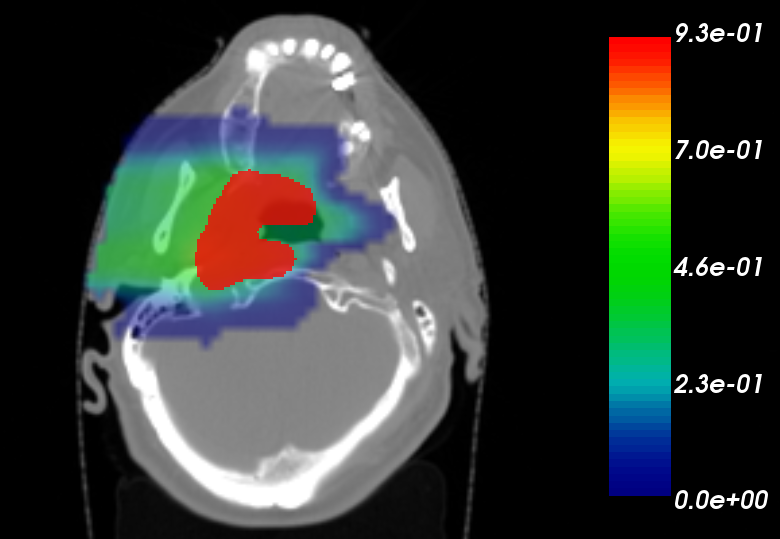
\includegraphics[width=0.5\linewidth]{ourpatient}
  \caption{A slice of the CT used in this study is shown with the dose due to field 2 of the plan overlaid, color scale in Grey, with in red the planned treatment volume (PTV).}
  \label{fig:our-patient}
\end{figure}

To study real patient change, a planning and replanning CT (CT and RPCT) set was chosen for a patient with a head and neck tumor, wrapped around the trachea. The CT and RPCT were co-registered on bony structures. A realistic two-field TP was created on the CT, and then simulated with Gate \citep{Grevillot2012}. In this paper, only the main field will be studied. The CT with the dose due to this field and the PTV structure are seen in fig.~\ref{fig:our-patient}.

%%%%%%%%%%%%%%%%%%%%%%%%%%%%%%%%%%%%%%%%%%%%%%%%%%%%%%%%%%%%%%%%%%%%%%%%%%%%%%%%
\subsection{Spot selection}

\begin{figure}[htp]
  \centering
  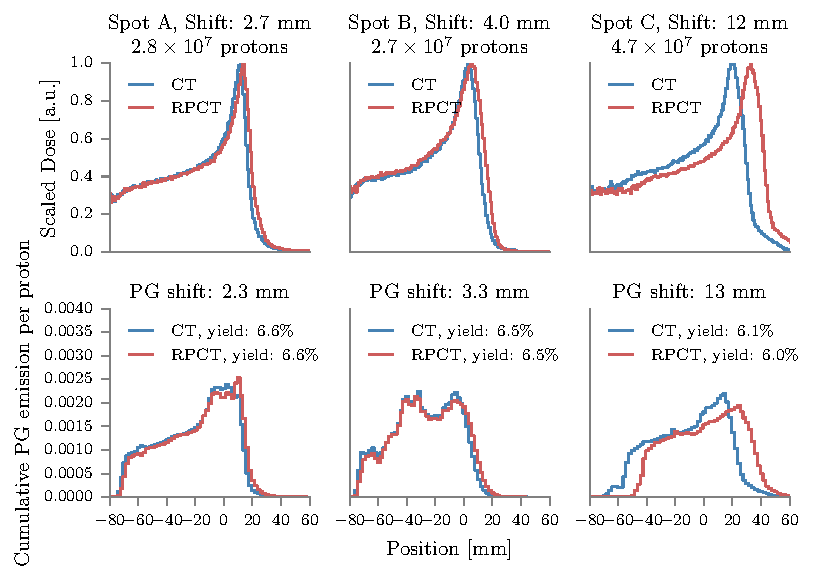
\includegraphics[width=0.99\linewidth]{spotprofiles}
  \caption{The three chosen spots, based on their shifts and quality of shift. Dose is normalized by mass, which explains the lack of structure. Top row: dose profiles, bottom row: PG emission profiles as used in the second stage of the simulation (PG detection). The yield is the integral yield of the whole image, so 6\% means 6 out of 100 protons generate a PG.}
  \label{fig:the-spots}
\end{figure}

\begin{table}
\centering
\begin{tabular}{llll}
	 & Spot A & Spot B & Spot C\\
	\midrule
	Dose shift [mm] & 2.77 & 4.08 & 12.4\\
	PG emission shift [mm] & 2.32 & 3.34 & 13.9\\
	\midrule
	Iso-energy layer [MeV] & 145.86 & 143.02 & 143.02 \\
	x-pos [mm] & -24.0 &  -24.0 &  -24.0 \\
	y-pos [mm] & 16.0 & 40.0 & -40.0 \\
	Nr. protons & $2.75\cdot10^7$ & $2.72\cdot10^7$ & $4.73\cdot10^7$ \\
\end{tabular}
\caption{Summary of the properties of the selected spots.}
\label{table:spotselec}
\end{table}

Three spots (table~\ref{table:spotselec}) were selected for presentation in this study. Spot C, with a large shift of over a centimeter with a whiff of overshoot: the beam partially exits the patient causing the distal elevation seen in figure~\ref{fig:the-spots}. An expected shift of over a centimeter should be reliably detectable for any PG camera. Spots A and B are more challenging; with expected shifts between 2 and 4 mm they represent a minimum shift that the PG cameras should be able to detect.



%%%%%%%%%%%%%%%%%%%%%%%%%%%%%%%%%%%%%%%%%%%%%%%%%%%%%%%%%%%%%%%%%%%%%%%%%%%%%%%%
\subsection{Verification of the cameras}

In \cite{Priegnitz2015} PG shifts due to beam energy shifts are studied for the KES camera: the \emph{detectability} of the fall-off as function of the number of primaries. Here that simulation was recreated: a mono-energetic beam shoots into a waterbox at two energies. 50 realizations are generated with a 139 MeV beam energy, and 50 realizations with 144 MeV. At $10^9$ primaries, the distributions are well separated with a shift of 8.3 mm (different from \cite{Priegnitz2015} because of the different material). In figure 13 in \cite{Perali2014} with $10^9$ primaries a standard deviation of 1.5 mm is obtained, while here 1.21 and 1.14 mm were obtained. It is sufficient agreement to be confident of our setup and further results.

The KES prototype's sensitivity to accurate positioning with respect to the expected FOP was elaborated upon in \citet[Section IV.A.3]{Sterpin2015}: the detector response is, due to the KES collimator, not linear as with a parallel slit collimator. In this study, to make the comparison as fair as possible and avoid any bias, alignment on the FOP specific for each spot was ensured as follows: the intermediate PG source image of vpgTLE (equivalent to the PG emission) was projected on the beam axis, and then convolved with a Gaussian of $\upsigma = 8.5$ mm, which corresponds to the point spread function (PSF) with a FWHM of 20 mm used in \cite{Priegnitz2015} to approximate the detected profiles from the emitted profile. These profiles will be referred to as "PG + PSF" profiles. As a matter of fact, the MPS prototype has roughly the same PSF as the KES prototype so that "PG + PSF" fall-off position can be considered as the expected position for both cameras.

To verify the implementation of the MPS camera, the precision on the FOP, obtained with the procedure outlined in the previous paragraph, is compared to earlier results. In the caption of figure 9 in \cite{Pinto2014a} it is stated that with $10^8$ primaries a standard deviation of 1.3 mm is obtained for the detector design used here, which is about 20\% different from the results obtained in this study: 1.63 and 1.54 mm.

\section{Results}

The first study is on the performance of the two collimated PG camera designs on a patient case with a CT and follow-up CT. Secondly, we investigate how two PG cameras perform as function of the number of primaries for a given spot. To conclude, we propose a new spot-summing method, we discuss why it is an improvement over iso-energy layer summing, and demonstrate its effect.

%%%%%%%%%%%%%%%%%%%%%%%%%%%%%%%%%%%%%%%%%%%%%%%%%%%%%%%%%%%%%%%%%%%%%%%%%%%%%%%%
\subsection{Weight-modulated single spot}

\begin{figure}[htp]
  \centering
  \includegraphics[width=.8\textwidth]{{{spotprofiles_results}}}
  \caption{The profiles of a selected realization with $10^9$ protons for both cameras are here shown for each spot (column-wise) and for the MPS and KES cameras (row-wise), with the fall-off position drawn as vertical lines. The detection yields are shown in the subplot titles. The windows were kept constant with respect to figure~\ref{fig:the-spots} to facilitate comparison. The MPS profiles are cropped to fit the window and the narrower field of view of the KES is easily visible.}
  \label{fig:spotmeasuredprofiles}
\end{figure}

\begin{figure}[htp]
  \centering
  \includegraphics[width=.8\textwidth]{{{spotresults}}}
  \caption{The mean and standard deviations on the FOP differences are plotted for the spots (column-wise) and for the MPS and KES cameras (row-wise). Per subplot, means and standard deviations are shown for $10^9$, the original spot weight, $10^8$, and $10^7$ primaries. In red, the dose shift is shown, the value which would be clinically relevant. Note that the error bars with the MPS at $10^7$ primaries are clipped. For the exact quantities, please see table~\ref{table:spots}.}
  \label{fig:spotshifts}
\end{figure}

The procedure outlined in section~\ref{figmerit} and demonstrated in the validation stage, is performed for all number of primaries, for both cameras, for spots A, B and C. Because of the extent of these results, only the profiles for $10^9$ primaries (smallest statistical fluctuations) are shown, in figure~\ref{fig:spotmeasuredprofiles}. The plots of the final results, the FOP shift distributions and their $\upmu_\Delta$, $\upsigma_\Delta$ and P$_\Delta$ are shown in figure \ref{fig:spotshifts}.

\begin{table}
\centering
\begin{tabular}{llll}
	 & Spot A shift [mm] & Spot B shift [mm] & Spot C shift [mm]\\
	\midrule
	Dose & 2.77 & 4.08 & 12.4\\
	PG emission & 2.32 & 3.34 & 13.9\\
	PG + PSF & 2.61 & 2.91 & 11.9\\
	$\upmu_\Delta$ MPS @ $10^9$      & 2.68$\pm$0.77 & 3.23$\pm$0.77 & 12.6$\pm$1.15 \\
	$\upmu_\Delta$ KES @ $10^9$      & 2.56$\pm$1.93 & 3.27$\pm$2.24 & 9.79$\pm$2.25 \\
	$\upmu_\Delta$ MPS @ spot weight & 2.51$\pm$4.05 & 3.76$\pm$4.36 & 12.5$\pm$4.73 \\
	$\upmu_\Delta$ KES @ spot weight & -1.2$\pm$28.9 & -0.2$\pm$28.9 & 4.30$\pm$26.2 \\
	\midrule
	 & Spot A P$_\Delta$ & Spot B P$_\Delta$ & Spot C P$_\Delta$\\
	\midrule
	P$_\Delta$ MPS @ $10^9$      & 99\%  & 99\% & 100\% \\
	P$_\Delta$ KES @ $10^9$      & 43\%  & 59\% & 99\% \\
	P$_\Delta$ MPS @ spot weight & 20\%  & 24\% & 96\% \\
	P$_\Delta$ KES @ spot weight & 1.9\% & 1.6\% & 1.4\% \\
	\midrule
	 & Spot A spot weight & Spot B spot weight & Spot C spot weight\\
	\midrule
	Nr. protons & $2.75\cdot10^7$ & $2.72\cdot10^7$ & $4.73\cdot10^7$ \\
\end{tabular}
\caption{Fall-off position shifts on the dose and PG emission profiles. With "PG + PSF" the FOP on the PG emission profile convolved with a Gaussian with a 20 mm FWHM is indicated. The geometric effect of the detector not measuring the PGs at emissions but at detection, approximated by the convolution, leads to up or downstream shifted FOPs.}
\label{table:spots}
\end{table}

Table~\ref{table:spots} summarizes the results relevant to the estimated shifts. With $10^9$ primaries, both cameras are within 2 mm of the "PG + PSF" emission shift, except the KES camera in Spot C. Here, when its $\upsigma_\Delta$ is considered, it is within one $\upsigma$ of the expected value. At the prescribed spot weights, the MPS still converges on the correct $\upmu_\Delta$, but the KES no longer. Considering that the $\upsigma_\Delta$ for the KES is on the order of a quarter of the FoV of the camera, it seems fair to draw the conclusion no correct FOPs are estimated at these spot weights.

Turning to P$_\Delta$ at $10^9$ primaries, we observe that the MPS performs very well: for any spot the probability that a single RPCT realization indicates a change from the CT is at least 99\%. The KES reaches the same probability only for the large shift of Spot C. At their planned spot weights, neither camera provides great results except for the MPS for Spot C: even though the precision is 4.73 mm, the size of the true shift is enough to keep the CT and RPCT FOP distributions separated enough to be 96\% certain a single measurement would have provided a clue that there was a significant shift. 

%%%%%%%%%%%%%%%%%%%%%%%%%%%%%%%%%%%%%%%%%%%%%%%%%%%%%%%%%%%%%%%%%%%%%%%%%%%%%%%%

\subsection{Spot grouping}

\begin{figure}[htp]
  \centering
  \includegraphics[width=.8\textwidth]{{{layerprofiles_results}}}
  \caption{The profiles of a selected realization with $10^9$ protons for both cameras are here shown for each spot (column-wise) and for the MPS and KES cameras (row-wise), with the fall-off position drawn as vertical lines. The detection yields are shown in the subplot titles. The windows were kept constant with respect to figure~\ref{fig:the-spots} to facilitate comparison. The MPS profiles are cropped to fit the window and the narrower field of view of the KES is easily visible. The colors this time do not refer to the CT and RPCT profiles, but the iso-energy (blue) and iso-depth (green) groupings. All profiles were obtained by irradiating the CT; the RPCT data were left out of the plot. For the spot C grouping, the effect of the iso-depth grouping having about 10\% fewer proton can directly be ascertained.}
  \label{fig:layermeasuredprofiles}
\end{figure}

Since spot-by-spot FOP shift measurements appear to be off the table, we can consider collecting data during the delivery of multiple spots. Based on the spot modulation analysis, the minimum proton count required should be no less than $10^9$ primaries. Spot C is part of the first iso-energy layer (counted down from highest energy) having at least $10^9$ protons. The geometric group is constructed by grouping spots with FOPs closest to Spot C's FOP until $10^9\pm5\%$ protons is reached. The final count is $1.07\cdot10^9$ and $0.98\cdot10^9$ protons in the iso-energy and iso-depth layers respectively. The plots of the profiles for the CTs are shown in figure~\ref{fig:layermeasuredprofiles}.

\begin{figure}[htp]
  \centering
  \includegraphics[width=.7\textwidth]{{{layerresults}}}
  \caption{The mean and standard deviations on the FOP differences are plotted for the spots groupings (column-wise) and for the MPS and KES cameras (row-wise). Per subplot, means and standard deviations are shown for iso-energy and iso-depth groupings. In red, the dose shift is shown, the value which would be clinically relevant. For the exact quantities, please see table~\ref{table:layerresults}.}
  \label{fig:groupingother}
\end{figure}

If we make the iso-depth and iso-energy groups based on spots A and B, the plots in figure~\ref{fig:groupingother} are obtained. The number of primaries per grouping are nearly identical between the groupings ($0.84\cdot10^9$ for the spot A groupings and $1.07\cdot10^9$ for the spot B groupings). The small shift of spot A translates to small shifts in the groupings, especially the iso-depth grouping. Here, the FOP shift is well within the precision of the KES camera, and so it clearly loses its power to discriminate the CT signal for the RPCT ($P_\Delta$ = 14\%). The MPS shows, apart from the iso-energy group about spot A, a slight improved on the $\upmu_\Delta$ when compared to the spot set to $10^9$ protons. For each camera and spot, the precision on the FOP difference ($\upmu_\Delta$) improves with iso-depth over iso-energy grouping.

\begin{table}
\centering
\begin{tabular}{lllllll}
	 & Spot A & & Spot B & & Spot C\\
	 & iso-energy & iso-depth & iso-energy & iso-depth & iso-energy & iso-depth \\
	\midrule
	Dose & 2.47 & 1.60 & 6.40 & 4.07 & 6.40 & 6.40 \\
	PG emission & 4.94 & 2.32 & 7.12 & 3.78 & 7.12 & 7.12 \\
	PG + PSF & 3.20 & 2.18 & 4.94 & 4.51 & 4.94 & 6.25 \\
	$\upmu_\Delta$ MPS & 3.13$\pm$1.16 & 2.18$\pm$0.89 & 4.82$\pm$1.00 & 3.67$\pm$0.96 & 4.72$\pm$1.17 & 5.77$\pm$1.05  \\
	$\upmu_\Delta$ KES & 4.20$\pm$3.61 & 1.80$\pm$2.55 & 4.90$\pm$3.38 & 3.75$\pm$2.71 & 4.15$\pm$3.82 & 5.15$\pm$2.87  \\
	\midrule
	P$_\Delta$ MPS & 96\% & 92\%  & 99\% & 99\%  & 99\% & 99\% \\
	P$_\Delta$ KES & 34\% & 14\%  & 54\% & 57\%  & 99\% & 99\%  \\
	%\midrule
	\midrule
	Nr. protons & $0.84\cdot10^9$ & $0.84\cdot10^9$ & $1.07\cdot10^9$ & $1.07\cdot10^9$ & $1.07\cdot10^9$ & $0.98\cdot10^9$ \\
\end{tabular}
\caption{Overview of the iso-energy versus iso-depth comparison: the accuracy can be gleaned by comparing the shifts, the probability of measuring the change is estimated with P$_\Delta$. All shifts are given in millimeters. The fact that the PG emission and dose shifts for Spot C are exactly the same with iso-energy and iso-depth grouping is purely fortuitous.}
\label{table:layerresults}
\end{table}

Observing table~\ref{table:layerresults}, the better FOP precision of the KES for iso-depth grouping is translated to a higher probability to measure a significant change: $\upmu_\Delta$ improved from 38\% to 75\%. Looking at the groupings for Spot B, we see that the PG + PSF convolution produces a very similar FOP difference, while the FOP at PG emission and dose are quite different.

%%%%%%%%%%%%%%%%%%%%%%%%%%%%%%%%%%%%%%%%%%%%%%%%%%%%%%%%%%%%%%%%%%%%%%%%%%%%%%%%
\section{Discussion}

The present study was performed to find which treatment parameters determine the feasibility of two PG camera prototypes under clinical conditions. In further study, criteria such as desired minimum detectable shift and P$_\Delta$ should be set, so that the minimum number of protons required and the optimal grouping methods can be determined, for a certain camera and a certain TP.

%%%%%%%%%%%%%%%%%%%%%%%%%%%%%%%%%%%%%%%%%%%%%%%%%%%%%%%%%%%%%%%%%%%%%%%%%%%%%%%%
\subsection{Spot C}

The lower detection yield for Spot C may seem puzzling at first, but may be explained with gamma attenuation in the patient. Spot B and C share a coordinate in the plane transverse to the beam, but differ because they are almost at opposite ends of the other dimension in the transverse plane, which puts Spot C about 5 cm deeper in the patient seen from the cameras point of view. \citet[Table 3]{Lin2016} presented some results with respect to attenuation: a 10 cm increase of path length in a PMMA target leads to a 24\% detection yield reduction with the MPS camera of that paper, and 39\% with their KES. This is coherent with the 2 MeV photon attenuation of ~40\% obtained from the total attenuation coefficient (NIST database).

Also for spot C, the two grouping methods show off well how a signal based on fewer primaries can still outperform a better signal. In fig.~\ref{fig:groupingother} we see that both cameras have a better precision with iso-depth grouping than iso-energy grouping, despite the reduction in the number of primary protons and the consequent lower fall-off yields seen in fig.~\ref{fig:layermeasuredprofiles} (right column).


%%%%%%%%%%%%%%%%%%%%%%%%%%%%%%%%%%%%%%%%%%%%%%%%%%%%%%%%%%%%%%%%%%%%%%%%%%%%%%%%
\subsection{Simulation limitations}

This study was performed in silico. We used Geant4's QGSP\_BIC\_HP\_EMY physicslist to produce the results. For Geant4 is it known that currently PG production is overestimated; about 30\% according to \cite{Pinto2016}. This means that the results presented here may be better than in reality. Secondly, the vpgTLE method was used, which only simulates PGs due to the primary protons; no background estimation is provided, which has not been subjected to calibration with empirical results in any case. The room and nozzle were not modeled. Nevertheless, background estimates were taken from the original papers, and they were both based on experimental measurement.

%%%%%%%%%%%%%%%%%%%%%%%%%%%%%%%%%%%%%%%%%%%%%%%%%%%%%%%%%%%%%%%%%%%%%%%%%%%%%%%%
\subsection{Multiple fields and FOP}

Range verification is useful for under- and overshoot detection. It does not provide checks for transverse error. If there is an organ at risk (OAR) right behind the (geometrically) distal layer, FOP verification would provide valuable information. The interplay between multiple fields is difficult to disentangle, because an overshoot in one field may be compensated by an undershoot in another field, but that was considered out of scope for this publication. For single field treatment plans, or perpendicular beams where under- and overshoot or not likely to compensate, FOP verification is easily understood.

We can expect different shifts due to the profile's various shapes, changing from spot to spot, and profile differences depending on the particular grouping. Adding the PSF blurs these features and -- apparently -- can alter the shift estimate. Range mixing is inherent to spot grouping, and therefore to altering the profile shape, so it is something to be aware of.

%%%%%%%%%%%%%%%%%%%%%%%%%%%%%%%%%%%%%%%%%%%%%%%%%%%%%%%%%%%%%%%%%%%%%%%%%%%%%%%%
\subsection{From FOP to Range to Profile measurement}

The FOP estimation algorithm presented here was not the primary focus of the study. Possibilities for improvement are likely. As far as these authors could establish, our method was broadly similar to procedures in other publications: a maximum and a floor are extracted from the (smoothed) profile, the difference of which is the FO. Then, the FOP is set to the position where the profile crosses the half-FOA threshold. This means such procedure is sensitive to the floor and maximum estimation. With low statistics, the peak may be misidentified at a noisy bin. For the KES, incorrect alignment to the expected FOP may lead to the background falling outside of the field of view and may lead to a misidentified floor. In the plan studied here, the width of the KES FO was about 4 cm. The angular resolution of collimated cameras implies some blurring and therefore broadening of the FO width. With a FoV of 10 cm and a possible forward shift of perhaps more than a cm (Spot C) it is not uncommon that little if any post BP floor is in the FoV. Taking care to center the camera at the expected FOP (by taking the FOP of the PG emission convolved with a PSF) proved essential for the KES results. The MPS has a clear advantage here.

As mentioned in section~\ref{sec:fopproc}, it is important to distinguish range from FOP estimation. True range estimation, determining a FIP as well as a FOP, might improve the quality of the results, because it would allow the clinician to distinguish morphological change from setup shifts. Both would still suffer from the sensitivity to peak and floor estimation. In \cite{Roellinghoff2014a} fitting to a reference profile was proposed. \cite{Gueth2013} provided a correlation at registration method where shifted profiles could be distinguished from changed profiles (or bad data). Since in clinical conditions, each spot would require its own reference, the challenge becomes sourcing the references. \cite{Schumann2016} demonstrated that a per-spot PG profile may be obtained by convoluting the per-spot dose profiles. A TPS might then provide such profiles as a matter of course, which would profile the per-spot reference needed. Such profile-matching might make features such as camelbacks and spots that, due to inhomogeneity, deposit their dose with a single range (in this study it was discovered that about ~10\% of all spots in the studied TP do not have a single well-defined range).

%%%%%%%%%%%%%%%%%%%%%%%%%%%%%%%%%%%%%%%%%%%%%%%%%%%%%%%%%%%%%%%%%%%%%%%%%%%%%%%%
\subsection{Improved Spot-grouping}

Initially a transverse threshold was planned to be included in the grouping procedure: it stands to reason that patient changes are not uniform in the plane transverse to the beam. However, the minimum statistics discovered in the modulated spot analysis proved implacable: this treatment plan prescribes a total of $2.76\cdot10^{10}$ protons, which divided by the $10^9$ protons needed for a reliable (but still not sub-mm accurate) measurement with the MPS camera, leaves us with about 27 possible groups, if spots are grouped only once. At the proximal and distal ends the FOPs are too spread out to preserve FOP sharpness, and in any case this leaves very little room to include both FOP and transverse proximity in the grouping algorithm. Grouping on transverse position only, e.g. integrating the signal over all spots at one transverse position, is not expected to provide an improved FOP estimate, since the highest energy would determine the (distal) FOP, while all the other spots will do no more than elevate the plateau region.

A more sophisticated grouping method may strike a better balance between proximity, both transverse and longitudinal, and proton count than what we were able to envisage. A fundamental inverse relationship between proton count and spot-pertinence remains: the spots at the fields edges, distal and transverse, are most pertinent to FOP detection, while simultaneously very spread out and therefore difficult to group due to \emph{range mixing}. Moreover, the difficulty of low spot weights may be expected to increase with a trend towards smaller spots in non-isocentric planning \citep{Grevillot2015}.

A possible alternative avenue involves identifying regions of expected deviation. In the contouring stage, areas could be grouped on likelihood of deformation, for instance lung or windpipe. A pre-grouping might then provide a set of spots that should correlate to under- or overshoot in the particular region. Perhaps the TPS could be made aware, and place weightier, but fewer, spots at the distal end of the sensitive area, so that PG FOP measurement is aided.

%%%%%%%%%%%%%%%%%%%%%%%%%%%%%%%%%%%%%%%%%%%%%%%%%%%%%%%%%%%%%%%%%%%%%%%%%%%%%%%%
\section{Conclusion}

The first start-to-end clinical simulations of a multi-parallel slit camera for Prompt Gamma detection was presented. In addition, the first head-to-head comparison of two collimated PG cameras under realistic conditions was shown here. Also, a new spot grouping method was proposed, based on the notion of iso-depth. A small study of clinical spot weights was performed. Finally, a figure of merit is presented that provides an estimate of the probability of a measured FOP falling within or outside of the expected mean $\pm 2\times$ standard deviation.

At the nominal spot weights, neither camera can be expected to measure a correct result. Typical spot weights are studied, and with a downward trend of spot weights for low tolerance plans, it seems unlikely the two PG cameras considered will be able to produce clinically relevant results on the spot level, without significant improvements. Spot grouping is a way to improve the statistics and enable millimetric precision of the FOP estimate. Two spot grouping methods are studied, and only for the KES camera did the precision on the FOP shift improve by using the new iso-depth grouping, which deserves further investigation. A better than two out of three likelyhood to obtain a meaningful indication of the shift (P$_\Delta$) is likely for both cameras, when using iso-depth spot grouping instead of grouping by iso-energy layer.

%%%%%%%%%%%%%%%%%%%%%%%%%%%%%%%%%%%%%%%%%%%%%%%%%%%%%%%%%%%%%%%%%%%%%%%%%%%%%%%%
\section{Acknowledgements}

This work was partly supported by SIRIC LYric Grant INCa-DGOS-4664, LABEX PRIMES (ANR-11-LABX-0063 / ANR-11-IDEX-0007) and Fondation ARC. The authors would like to thank Marie-Claude Biston, Thomas Baudier and Gloria Vilches-Freixas for their help finding the CT images and making the treatment plan. We also thank Erik Almhagen and Uppsala University Hospital, Sweden for the treatment plan data presented in this paper.

%%%%%%%%%%%%%%%%%%%%%%%%%%%%%%%%%%%%%%%%%%%%%%%%%%%%%%%%%%%%%%%%%%%%%%%%%%%%%%%%
\newpage
\begin{appendices}

%%%%%%%%%%%%%%%%%%%%%%%%%%%%%%%%%%%%%%%%%%%%%%%%%%%%%%%%%%%%%%%%%%%%%%%%%%%%%%%%

\section{Fall-off position estimation procedure}\label{sec:fopproc}

\begin{enumerate}[noitemsep]
\item The measured PG profile is smoothed and interpolated with a smoothing spline function:

\begin{equation}
\sum_{i=1}^n (y_i - \hat f(x_i))^2 + \lambda \int_{x_1}^{x_n} \hat f''(x)^2 \,dx
\end{equation}

where $y_i$ is the measured PG profile and $x_i$ the associated x-coordinates, $\hat f(x_i)$ the estimate smoothed spline function and $\lambda$ a smoothing parameter that determines the penalty for deviating from measurement in exchange for smoothness (second order derivatives are close to zero on smooth functions). $\lambda = 0$ produces a perfect spline fit to the data, while $\lambda \gg 1$ produces a horizontal line. We found that $\lambda = 2$ provided an acceptable trade-off between overfitting to noise and removing too many features, which tends to happen for low statistic measurements.
\item The obtained function is plotted for 1024 $x_j$, an number that provided a sufficiently high resolution. Any $f(x_j) < 0$ are set to $0$. 
\item The global maximum is found.
\item The baseline is set equal to the lowest 25\% of bins.
\item From the distal end backwards, the first maximum is taken as the distal most peak position, if it is above the threshold of 30\% of the difference between baseline and global maximum. If no such point is found, the global maximum is taken as the distal most maximum.
\item The fall-off amplitude (FOA) is set to the difference between the distal maximum and baseline: $FOA = max-baseline$. The FOP is obtained by traversing the smoothed profile from the distal end towards the peak until $y_j > \frac{1}{2}FOA$.
\end{enumerate}

The results of this procedure are illustrated in figure~\ref{fig:our-fit}. Every PG profile was estimated 50 times, and so we obtained 50 estimates for the FOP. It is assumed that the FOPs follow a Gaussian distribution, so the mean of the 50 realizations gives the best FOP estimate and the sigma gives the precision of the ability to estimate the best FOP. Comparing the 50 FOP estimates obtained from the CT with the 50 estimates obtained from the RPCT simulations, gives 2500 possible shift estimates. Again, the distribution of shifts should be centered at the true shift, while the sigma indicates how likely it is that this true shift is detected under the current conditions.

\begin{figure}[htp]
  \centering
  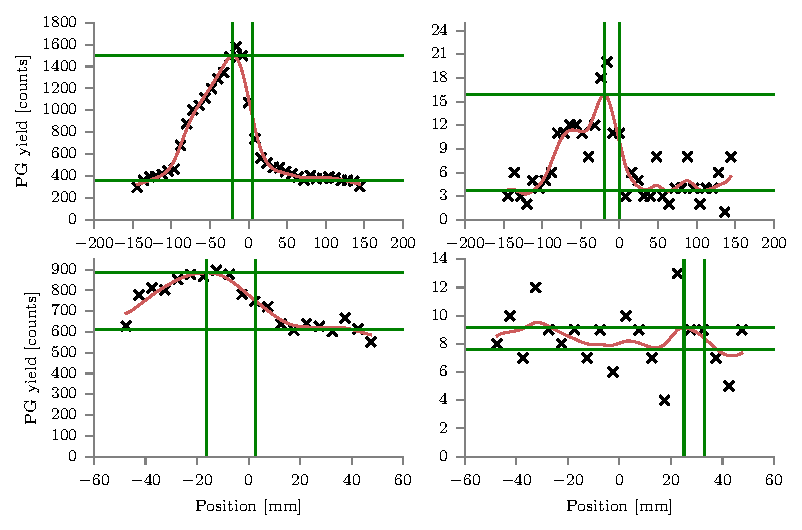
\includegraphics[width=0.9\linewidth]{fopproc}
  \caption{The top row demonstrates the fall-off determination procedure on the multi-parallel camera data; on the bottom row on knife-edge slit camera data. The left column is produced with a PG signal due to $10^9$ primaries, while the right column was produced with $10^7$ primary protons. In black crosses the measured PG counts are plotted. The smoothed data is shown in red. The green horizontal lines are drawn at the obtained distal maxima and baselines, while the vertical green lines shown the position of the distal maximum and the position of the fall-off. For the bottom-right plot, a history is visible where the procedure fails: the background induces an erroneous peak detection.}
  \label{fig:our-fit}
\end{figure}

%%%%%%%%%%%%%%%%%%%%%%%%%%%%%%%%%%%%%%%%%%%%%%%%%%%%%%%%%%%%%%%%%%%%%%%%%%%%%%%%
\end{appendices}
\newpage

%%%%%%%%%%%%%%%%%%%%%%%%%%%%%%%%%%%%%%%%%%%%%%%%%%%%%%%%%%%%%%%%%%%%%%%%%%%%%%%%

\bibliographystyle{plainnat}
\bibliography{../library.bib}
\end{document}%\grid
